\documentclass[twoside]{book}

% Packages required by doxygen
\usepackage{fixltx2e}
\usepackage{calc}
\usepackage{doxygen}
\usepackage{graphicx}
\usepackage[utf8]{inputenc}
\usepackage{makeidx}
\usepackage{multicol}
\usepackage{multirow}
\PassOptionsToPackage{warn}{textcomp}
\usepackage{textcomp}
\usepackage[nointegrals]{wasysym}
\usepackage[table]{xcolor}

% Font selection
\usepackage[T1]{fontenc}
\usepackage[scaled=.90]{helvet}
\usepackage{courier}
\usepackage{amssymb}
\usepackage{sectsty}
\renewcommand{\familydefault}{\sfdefault}
\allsectionsfont{%
  \fontseries{bc}\selectfont%
  \color{darkgray}%
}
\renewcommand{\DoxyLabelFont}{%
  \fontseries{bc}\selectfont%
  \color{darkgray}%
}
\newcommand{\+}{\discretionary{\mbox{\scriptsize$\hookleftarrow$}}{}{}}

% Page & text layout
\usepackage{geometry}
\geometry{%
  a4paper,%
  top=2.5cm,%
  bottom=2.5cm,%
  left=2.5cm,%
  right=2.5cm%
}
\tolerance=750
\hfuzz=15pt
\hbadness=750
\setlength{\emergencystretch}{15pt}
\setlength{\parindent}{0cm}
\setlength{\parskip}{0.2cm}
\makeatletter
\renewcommand{\paragraph}{%
  \@startsection{paragraph}{4}{0ex}{-1.0ex}{1.0ex}{%
    \normalfont\normalsize\bfseries\SS@parafont%
  }%
}
\renewcommand{\subparagraph}{%
  \@startsection{subparagraph}{5}{0ex}{-1.0ex}{1.0ex}{%
    \normalfont\normalsize\bfseries\SS@subparafont%
  }%
}
\makeatother

% Headers & footers
\usepackage{fancyhdr}
\pagestyle{fancyplain}
\fancyhead[LE]{\fancyplain{}{\bfseries\thepage}}
\fancyhead[CE]{\fancyplain{}{}}
\fancyhead[RE]{\fancyplain{}{\bfseries\leftmark}}
\fancyhead[LO]{\fancyplain{}{\bfseries\rightmark}}
\fancyhead[CO]{\fancyplain{}{}}
\fancyhead[RO]{\fancyplain{}{\bfseries\thepage}}
\fancyfoot[LE]{\fancyplain{}{}}
\fancyfoot[CE]{\fancyplain{}{}}
\fancyfoot[RE]{\fancyplain{}{\bfseries\scriptsize Generated on Thu Dec 4 2014 16\+:27\+:55 for My Project by Doxygen }}
\fancyfoot[LO]{\fancyplain{}{\bfseries\scriptsize Generated on Thu Dec 4 2014 16\+:27\+:55 for My Project by Doxygen }}
\fancyfoot[CO]{\fancyplain{}{}}
\fancyfoot[RO]{\fancyplain{}{}}
\renewcommand{\footrulewidth}{0.4pt}
\renewcommand{\chaptermark}[1]{%
  \markboth{#1}{}%
}
\renewcommand{\sectionmark}[1]{%
  \markright{\thesection\ #1}%
}

% Indices & bibliography
\usepackage{natbib}
\usepackage[titles]{tocloft}
\setcounter{tocdepth}{3}
\setcounter{secnumdepth}{5}
\makeindex

% Hyperlinks (required, but should be loaded last)
\usepackage{ifpdf}
\ifpdf
  \usepackage[pdftex,pagebackref=true]{hyperref}
\else
  \usepackage[ps2pdf,pagebackref=true]{hyperref}
\fi
\hypersetup{%
  colorlinks=true,%
  linkcolor=blue,%
  citecolor=blue,%
  unicode%
}

% Custom commands
\newcommand{\clearemptydoublepage}{%
  \newpage{\pagestyle{empty}\cleardoublepage}%
}


%===== C O N T E N T S =====

\begin{document}

% Titlepage & ToC
\hypersetup{pageanchor=false,
             bookmarks=true,
             bookmarksnumbered=true,
             pdfencoding=unicode
            }
\pagenumbering{roman}
\begin{titlepage}
\vspace*{7cm}
\begin{center}%
{\Large My Project }\\
\vspace*{1cm}
{\large Generated by Doxygen 1.8.8}\\
\vspace*{0.5cm}
{\small Thu Dec 4 2014 16:27:55}\\
\end{center}
\end{titlepage}
\clearemptydoublepage
\tableofcontents
\clearemptydoublepage
\pagenumbering{arabic}
\hypersetup{pageanchor=true}

%--- Begin generated contents ---
\chapter{Hierarchical Index}
\section{Class Hierarchy}
This inheritance list is sorted roughly, but not completely, alphabetically\+:\begin{DoxyCompactList}
\item Mono\+Behaviour\begin{DoxyCompactList}
\item \contentsline{section}{box}{\pageref{classbox}}{}
\item \contentsline{section}{button\+Play}{\pageref{classbutton_play}}{}
\item \contentsline{section}{collision}{\pageref{classcollision}}{}
\item \contentsline{section}{gravity\+Shift}{\pageref{classgravity_shift}}{}
\item \contentsline{section}{Level\+Select}{\pageref{class_level_select}}{}
\item \contentsline{section}{Robot\+Controller\+Sript}{\pageref{class_robot_controller_sript}}{}
\item \contentsline{section}{Robot\+L\+E\+F\+T}{\pageref{class_robot_l_e_f_t}}{}
\item \contentsline{section}{Robot\+U\+P}{\pageref{class_robot_u_p}}{}
\item \contentsline{section}{trigger}{\pageref{classtrigger}}{}
\item \contentsline{section}{U\+I\+Manager}{\pageref{class_u_i_manager}}{}
\item \contentsline{section}{win}{\pageref{classwin}}{}
\end{DoxyCompactList}
\end{DoxyCompactList}

\chapter{Class Index}
\section{Class List}
Here are the classes, structs, unions and interfaces with brief descriptions\+:\begin{DoxyCompactList}
\item\contentsline{section}{\hyperlink{classbox}{box} }{\pageref{classbox}}{}
\item\contentsline{section}{\hyperlink{classbutton_play}{button\+Play} }{\pageref{classbutton_play}}{}
\item\contentsline{section}{\hyperlink{classcollision}{collision} }{\pageref{classcollision}}{}
\item\contentsline{section}{\hyperlink{classgravity_shift}{gravity\+Shift} }{\pageref{classgravity_shift}}{}
\item\contentsline{section}{\hyperlink{class_level_select}{Level\+Select} }{\pageref{class_level_select}}{}
\item\contentsline{section}{\hyperlink{class_robot_controller_sript}{Robot\+Controller\+Sript} }{\pageref{class_robot_controller_sript}}{}
\item\contentsline{section}{\hyperlink{class_robot_l_e_f_t}{Robot\+L\+E\+F\+T} }{\pageref{class_robot_l_e_f_t}}{}
\item\contentsline{section}{\hyperlink{class_robot_u_p}{Robot\+U\+P} }{\pageref{class_robot_u_p}}{}
\item\contentsline{section}{\hyperlink{classtrigger}{trigger} }{\pageref{classtrigger}}{}
\item\contentsline{section}{\hyperlink{class_u_i_manager}{U\+I\+Manager} }{\pageref{class_u_i_manager}}{}
\item\contentsline{section}{\hyperlink{classwin}{win} }{\pageref{classwin}}{}
\end{DoxyCompactList}

\chapter{File Index}
\section{File List}
Here is a list of all documented files with brief descriptions\+:\begin{DoxyCompactList}
\item\contentsline{section}{\hyperlink{trigger_8cs}{trigger.\+cs} }{\pageref{trigger_8cs}}{}
\item\contentsline{section}{\hyperlink{win_8cs}{win.\+cs} }{\pageref{win_8cs}}{}
\end{DoxyCompactList}

\chapter{Class Documentation}
\hypertarget{classbox}{}\section{box Class Reference}
\label{classbox}\index{box@{box}}
Inheritance diagram for box\+:\begin{figure}[H]
\begin{center}
\leavevmode
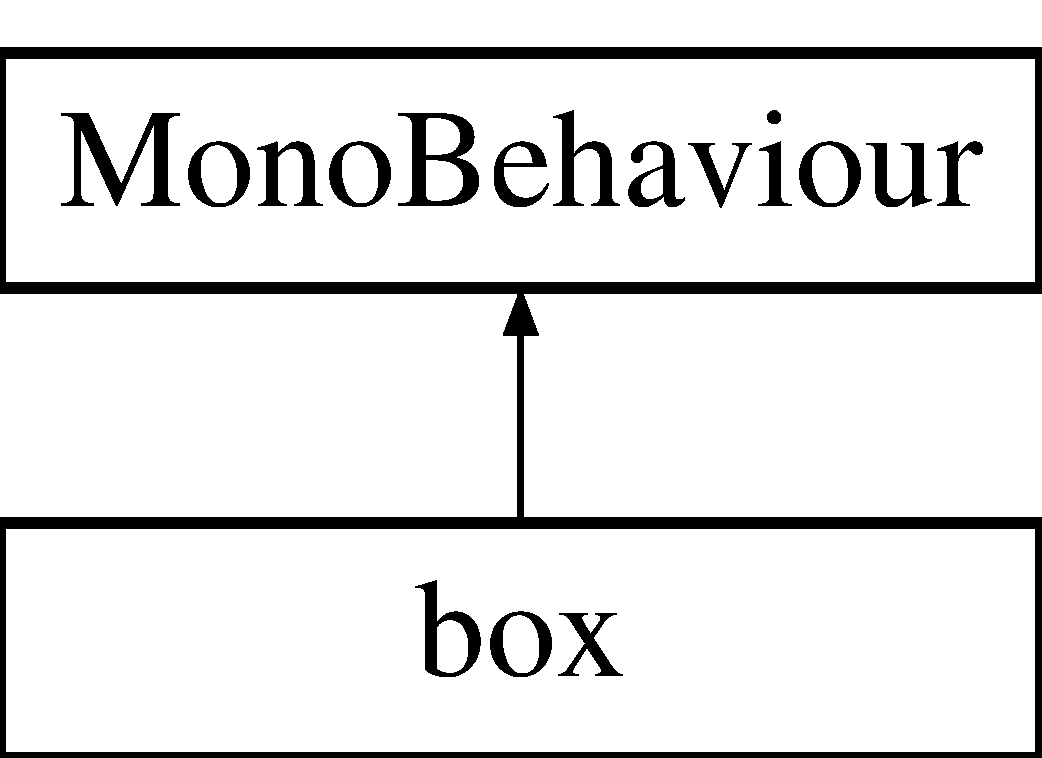
\includegraphics[height=2.000000cm]{classbox}
\end{center}
\end{figure}


The documentation for this class was generated from the following file\+:\begin{DoxyCompactItemize}
\item 
box.\+cs\end{DoxyCompactItemize}

\hypertarget{classbutton_play}{}\section{button\+Play Class Reference}
\label{classbutton_play}\index{button\+Play@{button\+Play}}
Inheritance diagram for button\+Play\+:\begin{figure}[H]
\begin{center}
\leavevmode
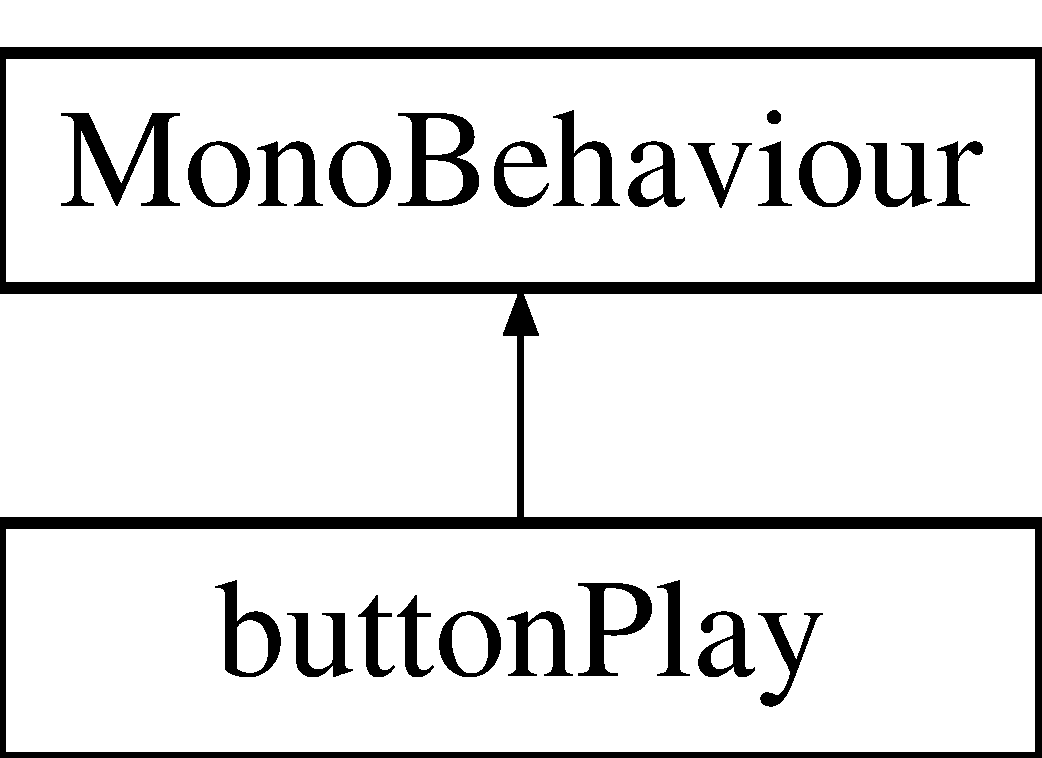
\includegraphics[height=2.000000cm]{classbutton_play}
\end{center}
\end{figure}
\subsection*{Public Attributes}
\begin{DoxyCompactItemize}
\item 
\hypertarget{classbutton_play_a03701ef5298febd01be36db9deda4529}{}Game\+Object {\bfseries Play}\label{classbutton_play_a03701ef5298febd01be36db9deda4529}

\item 
\hypertarget{classbutton_play_ac0f36b557664e8684cd2dac89ae522ae}{}Game\+Object {\bfseries Levels}\label{classbutton_play_ac0f36b557664e8684cd2dac89ae522ae}

\item 
\hypertarget{classbutton_play_aebcf3ac5bb08658d870e6b8e2e60f24a}{}Game\+Object {\bfseries Credits}\label{classbutton_play_aebcf3ac5bb08658d870e6b8e2e60f24a}

\end{DoxyCompactItemize}


The documentation for this class was generated from the following file\+:\begin{DoxyCompactItemize}
\item 
button\+Play.\+cs\end{DoxyCompactItemize}

\hypertarget{classcollision}{}\section{collision Class Reference}
\label{classcollision}\index{collision@{collision}}
Inheritance diagram for collision\+:\begin{figure}[H]
\begin{center}
\leavevmode
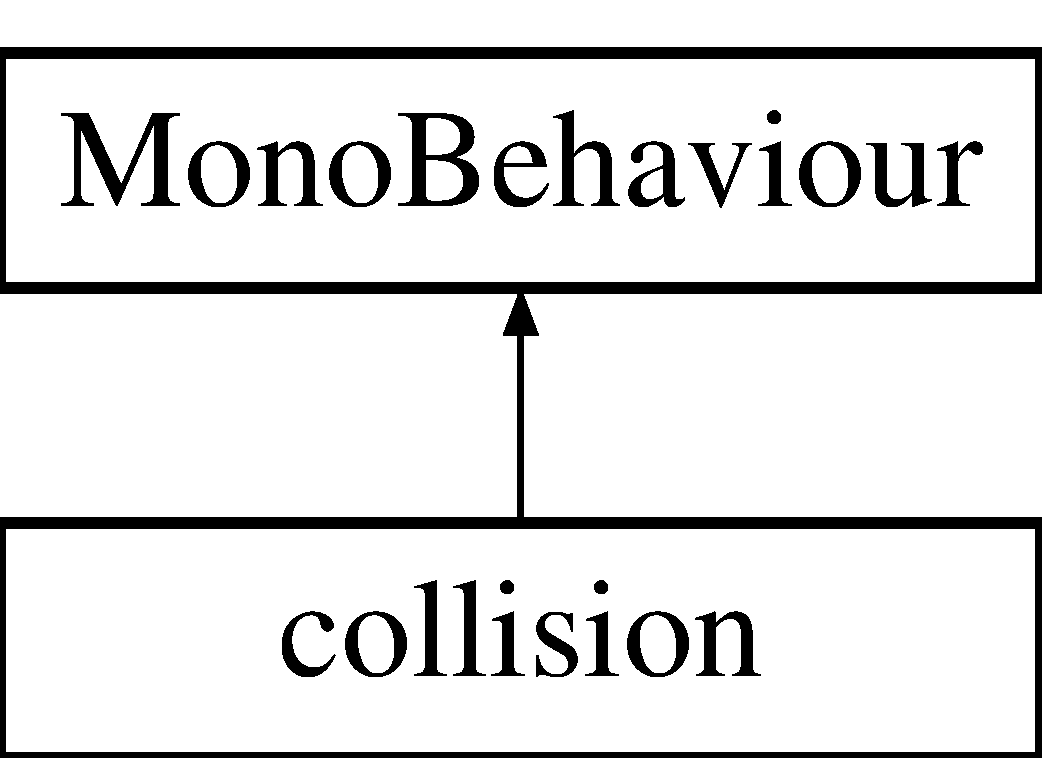
\includegraphics[height=2.000000cm]{classcollision}
\end{center}
\end{figure}


The documentation for this class was generated from the following file\+:\begin{DoxyCompactItemize}
\item 
collision.\+cs\end{DoxyCompactItemize}

\hypertarget{classgravity_shift}{}\section{gravity\+Shift Class Reference}
\label{classgravity_shift}\index{gravity\+Shift@{gravity\+Shift}}
Inheritance diagram for gravity\+Shift\+:\begin{figure}[H]
\begin{center}
\leavevmode
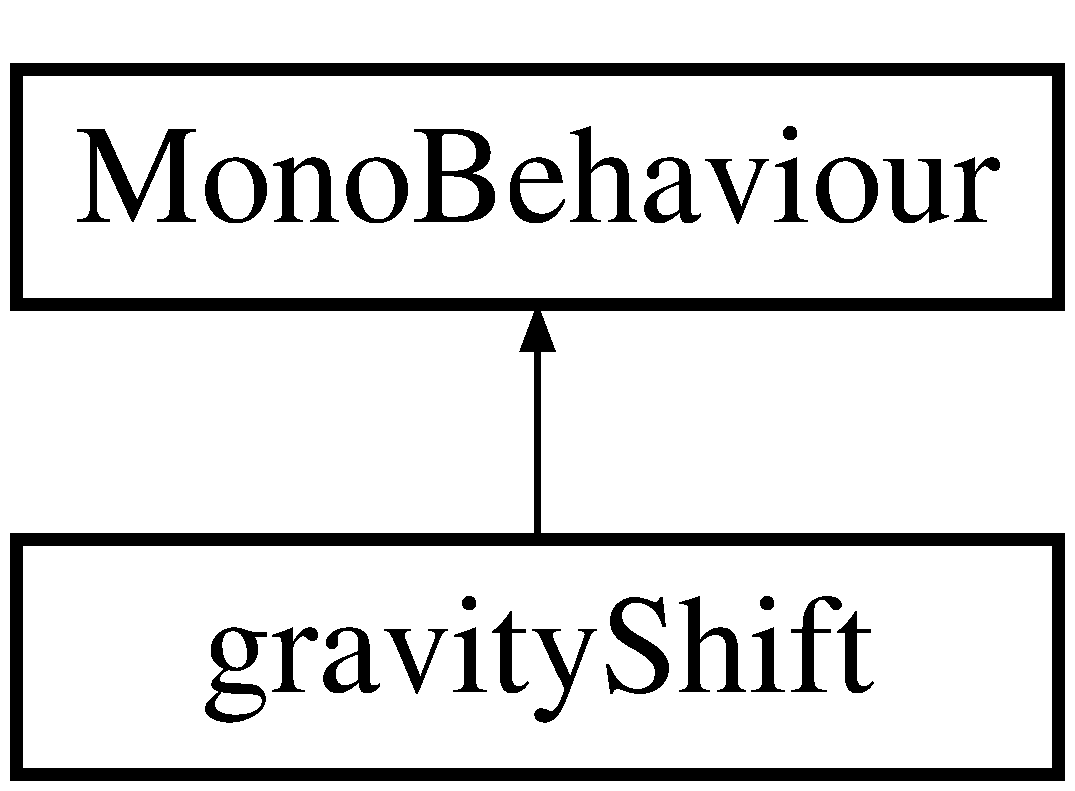
\includegraphics[height=2.000000cm]{classgravity_shift}
\end{center}
\end{figure}


The documentation for this class was generated from the following file\+:\begin{DoxyCompactItemize}
\item 
gravity\+Shift.\+cs\end{DoxyCompactItemize}

\hypertarget{class_level_select}{}\section{Level\+Select Class Reference}
\label{class_level_select}\index{Level\+Select@{Level\+Select}}
Inheritance diagram for Level\+Select\+:\begin{figure}[H]
\begin{center}
\leavevmode
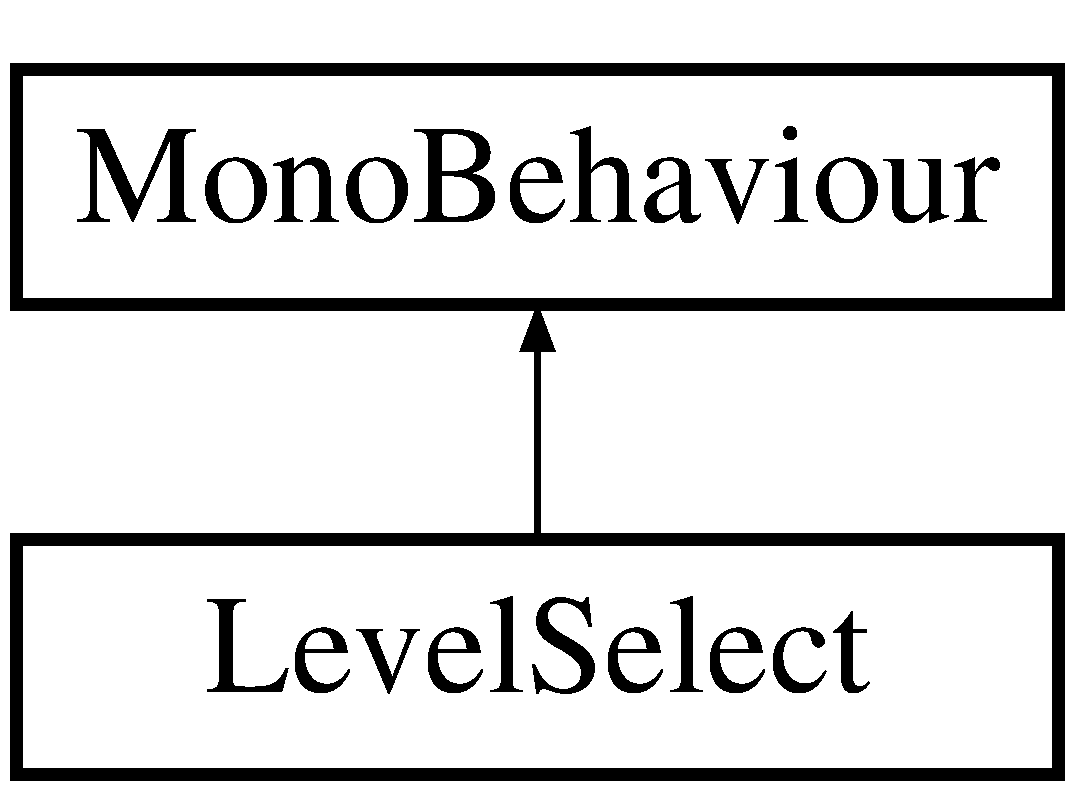
\includegraphics[height=2.000000cm]{class_level_select}
\end{center}
\end{figure}


The documentation for this class was generated from the following file\+:\begin{DoxyCompactItemize}
\item 
Level\+Select.\+cs\end{DoxyCompactItemize}

\hypertarget{class_robot_controller_sript}{}\section{Robot\+Controller\+Sript Class Reference}
\label{class_robot_controller_sript}\index{Robot\+Controller\+Sript@{Robot\+Controller\+Sript}}
Inheritance diagram for Robot\+Controller\+Sript\+:\begin{figure}[H]
\begin{center}
\leavevmode
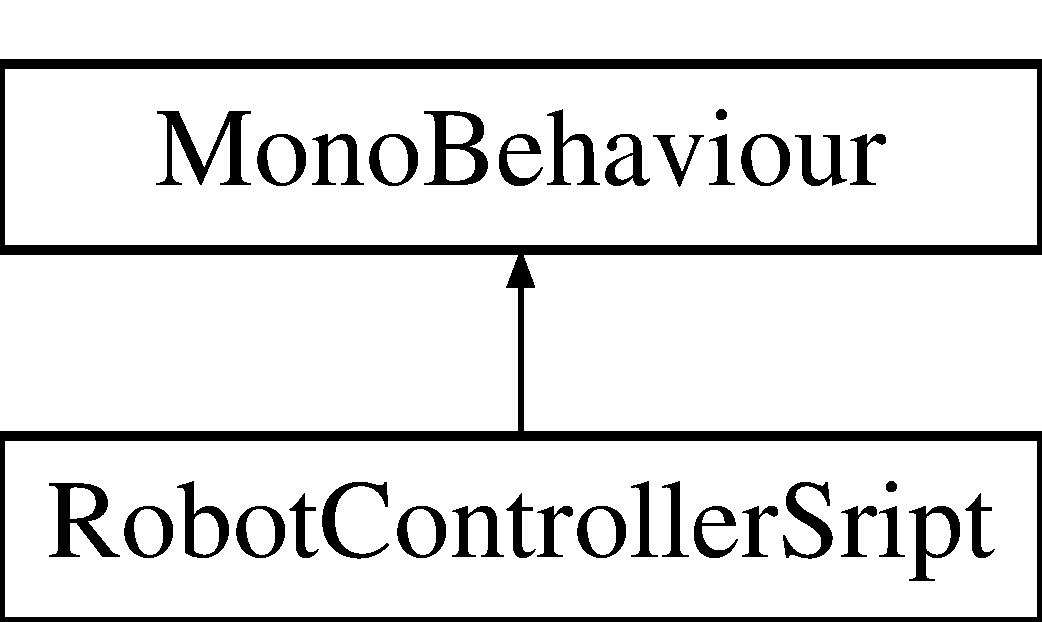
\includegraphics[height=2.000000cm]{class_robot_controller_sript}
\end{center}
\end{figure}
\subsection*{Public Attributes}
\begin{DoxyCompactItemize}
\item 
\hypertarget{class_robot_controller_sript_afc3d6129088b04b7201251e36cc395f8}{}float {\bfseries max\+Speed} = 10f\label{class_robot_controller_sript_afc3d6129088b04b7201251e36cc395f8}

\item 
\hypertarget{class_robot_controller_sript_a94b64fa5463dff9f47e8b343c51664cf}{}Transform {\bfseries ground\+Check}\label{class_robot_controller_sript_a94b64fa5463dff9f47e8b343c51664cf}

\item 
\hypertarget{class_robot_controller_sript_a532838fbb2f95bf6f8f4c177058d00c5}{}Layer\+Mask {\bfseries what\+Is\+Ground}\label{class_robot_controller_sript_a532838fbb2f95bf6f8f4c177058d00c5}

\item 
\hypertarget{class_robot_controller_sript_a44f7b8532b8e9259f7e1d3243e650914}{}float {\bfseries jump\+Force} = 700f\label{class_robot_controller_sript_a44f7b8532b8e9259f7e1d3243e650914}

\item 
\hypertarget{class_robot_controller_sript_ab00409bc1b9b249cebcd04228c12eaeb}{}int {\bfseries jumpdir}\label{class_robot_controller_sript_ab00409bc1b9b249cebcd04228c12eaeb}

\item 
\hypertarget{class_robot_controller_sript_ae98a4119e477ff872c360ca4a1436dc3}{}Audio\+Clip {\bfseries crush}\label{class_robot_controller_sript_ae98a4119e477ff872c360ca4a1436dc3}

\end{DoxyCompactItemize}


The documentation for this class was generated from the following file\+:\begin{DoxyCompactItemize}
\item 
Robot\+Controller\+Sript.\+cs\end{DoxyCompactItemize}

\hypertarget{class_robot_l_e_f_t}{}\section{Robot\+L\+E\+F\+T Class Reference}
\label{class_robot_l_e_f_t}\index{Robot\+L\+E\+F\+T@{Robot\+L\+E\+F\+T}}
Inheritance diagram for Robot\+L\+E\+F\+T\+:\begin{figure}[H]
\begin{center}
\leavevmode
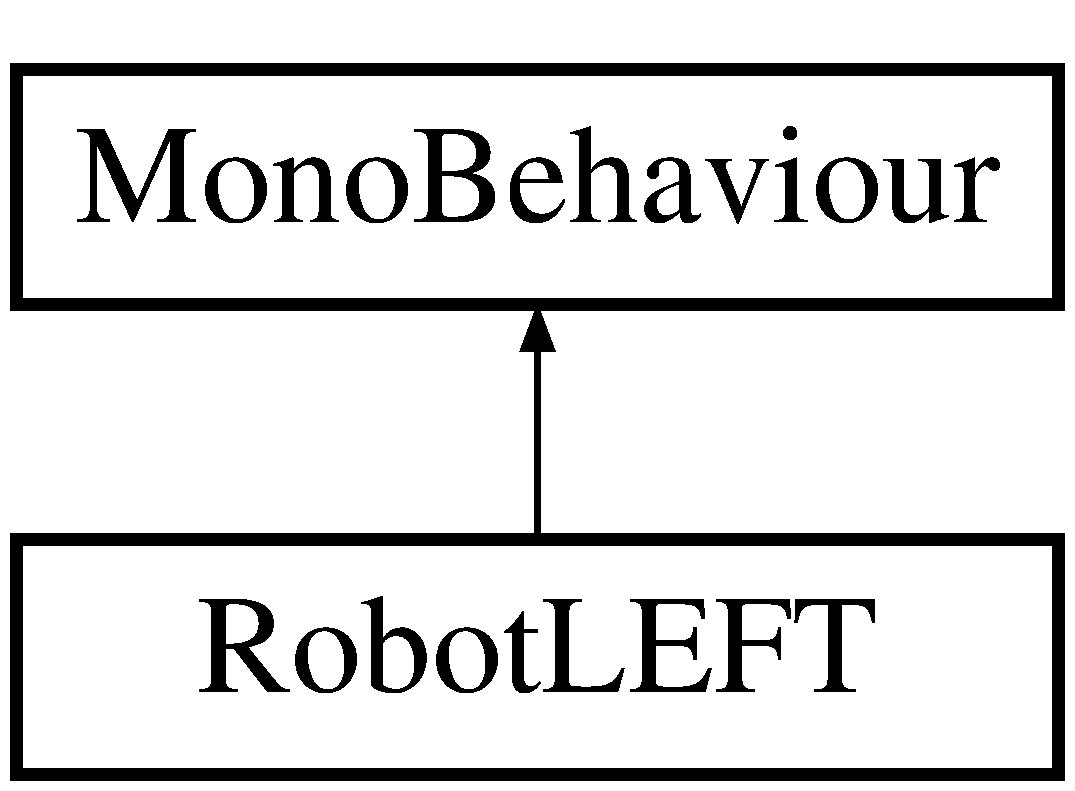
\includegraphics[height=2.000000cm]{class_robot_l_e_f_t}
\end{center}
\end{figure}
\subsection*{Public Attributes}
\begin{DoxyCompactItemize}
\item 
\hypertarget{class_robot_l_e_f_t_ab50adc52a29d0feb58e66abcd81d2036}{}float {\bfseries max\+Speed} = 10f\label{class_robot_l_e_f_t_ab50adc52a29d0feb58e66abcd81d2036}

\item 
\hypertarget{class_robot_l_e_f_t_add4b25dbcf5341aa3bd3113aac63c30c}{}Transform {\bfseries ground\+Check}\label{class_robot_l_e_f_t_add4b25dbcf5341aa3bd3113aac63c30c}

\item 
\hypertarget{class_robot_l_e_f_t_a1f338d3efc92bcb00ea70954912b83ef}{}Layer\+Mask {\bfseries what\+Is\+Ground}\label{class_robot_l_e_f_t_a1f338d3efc92bcb00ea70954912b83ef}

\item 
\hypertarget{class_robot_l_e_f_t_a2d0a0a4d8d9430fbbc0555d892d9c20e}{}float {\bfseries jump\+Force} = 700f\label{class_robot_l_e_f_t_a2d0a0a4d8d9430fbbc0555d892d9c20e}

\item 
\hypertarget{class_robot_l_e_f_t_ad6f03773c7872e13ae9a61fde7624c79}{}int {\bfseries jumpdir}\label{class_robot_l_e_f_t_ad6f03773c7872e13ae9a61fde7624c79}

\item 
\hypertarget{class_robot_l_e_f_t_aec8e155a3b82394c81ecb8eeca6ae8b6}{}Audio\+Clip {\bfseries crush}\label{class_robot_l_e_f_t_aec8e155a3b82394c81ecb8eeca6ae8b6}

\end{DoxyCompactItemize}


The documentation for this class was generated from the following file\+:\begin{DoxyCompactItemize}
\item 
Robot\+L\+E\+F\+T.\+cs\end{DoxyCompactItemize}

\hypertarget{class_robot_u_p}{}\section{Robot\+U\+P Class Reference}
\label{class_robot_u_p}\index{Robot\+U\+P@{Robot\+U\+P}}
Inheritance diagram for Robot\+U\+P\+:\begin{figure}[H]
\begin{center}
\leavevmode
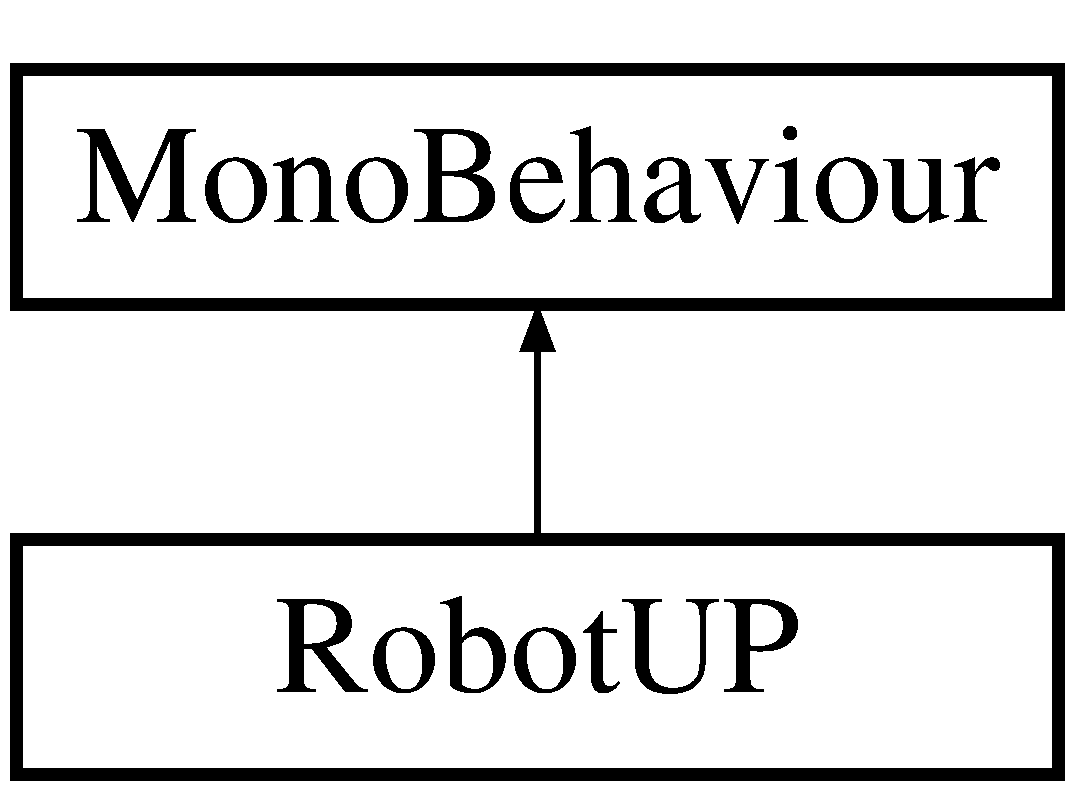
\includegraphics[height=2.000000cm]{class_robot_u_p}
\end{center}
\end{figure}
\subsection*{Public Attributes}
\begin{DoxyCompactItemize}
\item 
\hypertarget{class_robot_u_p_adaa4938db69717a593c24fb080c9a0b2}{}float {\bfseries max\+Speed} = 10f\label{class_robot_u_p_adaa4938db69717a593c24fb080c9a0b2}

\item 
\hypertarget{class_robot_u_p_a788f69026ec7cb861c976f48ed173e3f}{}Transform {\bfseries ground\+Check}\label{class_robot_u_p_a788f69026ec7cb861c976f48ed173e3f}

\item 
\hypertarget{class_robot_u_p_af65f8e27eb07754fb31db01e2ae70ff2}{}Layer\+Mask {\bfseries what\+Is\+Ground}\label{class_robot_u_p_af65f8e27eb07754fb31db01e2ae70ff2}

\item 
\hypertarget{class_robot_u_p_a76a553f3d94cc791cd1f9564c4e305a1}{}float {\bfseries jump\+Force} = 700f\label{class_robot_u_p_a76a553f3d94cc791cd1f9564c4e305a1}

\item 
\hypertarget{class_robot_u_p_afd687df4e7449818d7ecaa6a02930193}{}int {\bfseries jumpdir}\label{class_robot_u_p_afd687df4e7449818d7ecaa6a02930193}

\item 
\hypertarget{class_robot_u_p_ada3f9b6c3dfd5eca37f091eb82c1bea6}{}Audio\+Clip {\bfseries crush}\label{class_robot_u_p_ada3f9b6c3dfd5eca37f091eb82c1bea6}

\end{DoxyCompactItemize}


The documentation for this class was generated from the following file\+:\begin{DoxyCompactItemize}
\item 
Robot\+U\+P.\+cs\end{DoxyCompactItemize}

\hypertarget{classtrigger}{}\section{trigger Class Reference}
\label{classtrigger}\index{trigger@{trigger}}
Inheritance diagram for trigger\+:\begin{figure}[H]
\begin{center}
\leavevmode
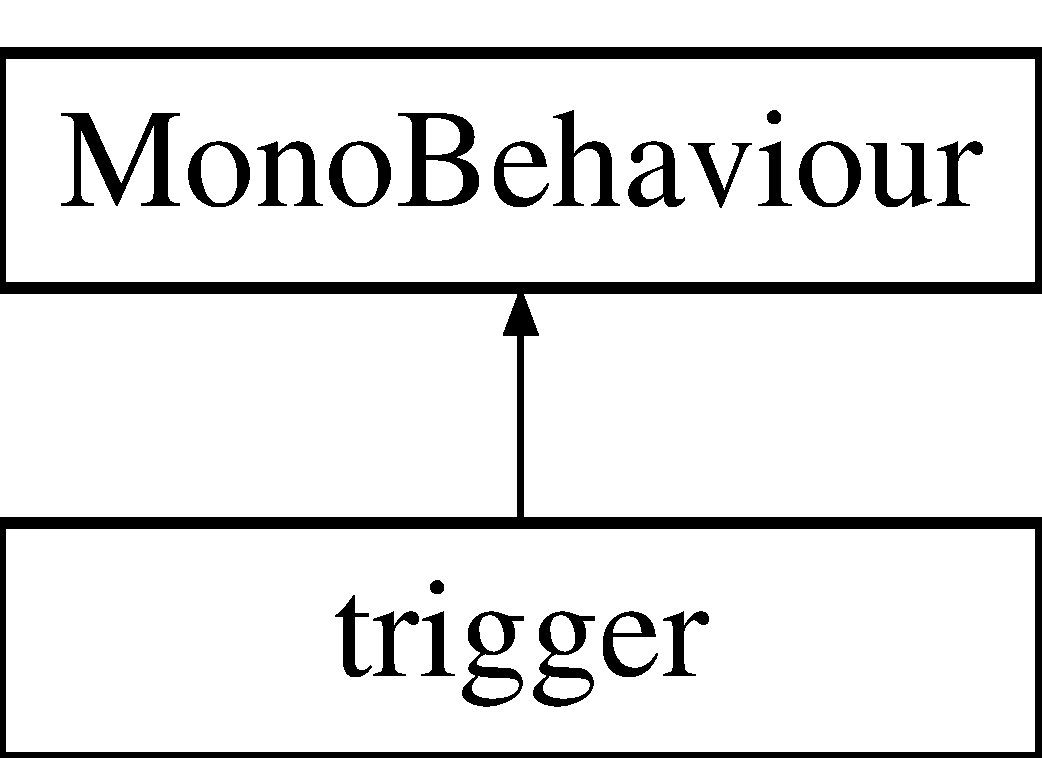
\includegraphics[height=2.000000cm]{classtrigger}
\end{center}
\end{figure}
\subsection*{Public Attributes}
\begin{DoxyCompactItemize}
\item 
\hypertarget{classtrigger_a63c64e0345e9d2ef9423d8861d94f741}{}Game\+Object {\bfseries moving\+Wall}\label{classtrigger_a63c64e0345e9d2ef9423d8861d94f741}

\item 
\hypertarget{classtrigger_ac114f0bc7c9c656b97fb3dc0c06be5f7}{}string {\bfseries door\+Open}\label{classtrigger_ac114f0bc7c9c656b97fb3dc0c06be5f7}

\item 
\hypertarget{classtrigger_a73e0a60c442d52c1b5a9cdcb8ab34ddb}{}Game\+Object {\bfseries success}\label{classtrigger_a73e0a60c442d52c1b5a9cdcb8ab34ddb}

\item 
\hypertarget{classtrigger_a4d7387fc565a240628c0d63303489129}{}Game\+Object {\bfseries elect1}\label{classtrigger_a4d7387fc565a240628c0d63303489129}

\item 
\hypertarget{classtrigger_af4d9cfb5fed1a0736c0679385bea4c57}{}Game\+Object {\bfseries elect2}\label{classtrigger_af4d9cfb5fed1a0736c0679385bea4c57}

\item 
\hypertarget{classtrigger_abdaf36361a49e8b1eea5053147e5de9d}{}Audio\+Clip {\bfseries Zap}\label{classtrigger_abdaf36361a49e8b1eea5053147e5de9d}

\end{DoxyCompactItemize}


The documentation for this class was generated from the following file\+:\begin{DoxyCompactItemize}
\item 
\hyperlink{trigger_8cs}{trigger.\+cs}\end{DoxyCompactItemize}

\hypertarget{class_u_i_manager}{}\section{U\+I\+Manager Class Reference}
\label{class_u_i_manager}\index{U\+I\+Manager@{U\+I\+Manager}}
Inheritance diagram for U\+I\+Manager\+:\begin{figure}[H]
\begin{center}
\leavevmode
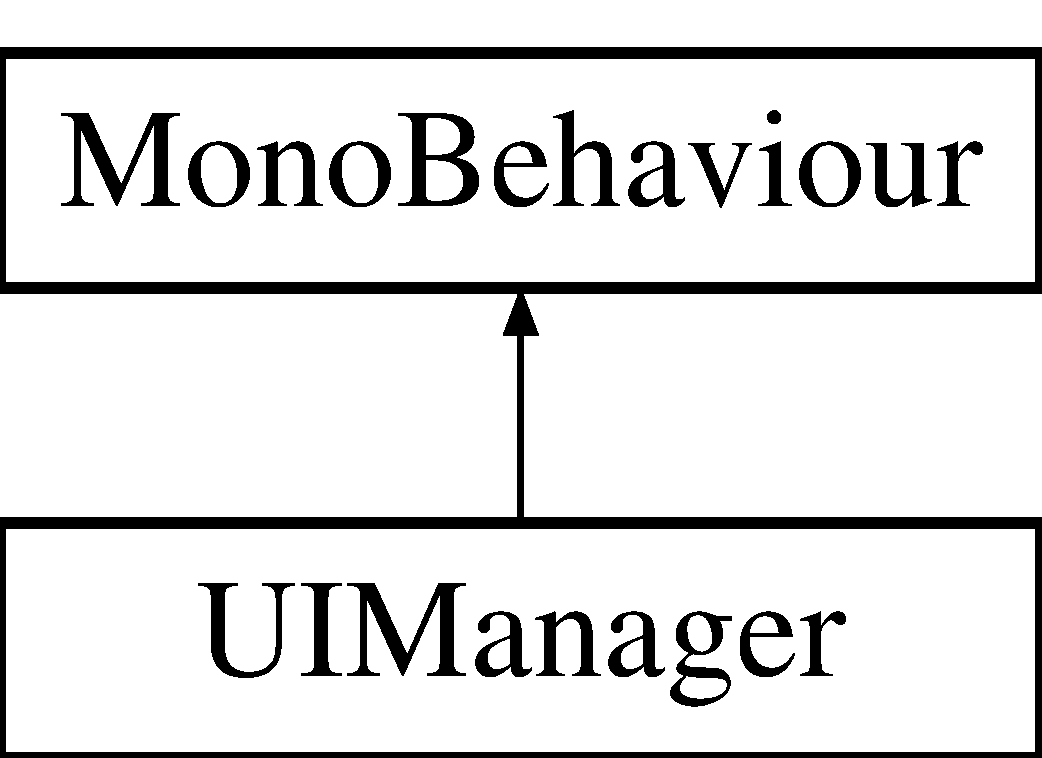
\includegraphics[height=2.000000cm]{class_u_i_manager}
\end{center}
\end{figure}
\subsection*{Public Member Functions}
\begin{DoxyCompactItemize}
\item 
\hypertarget{class_u_i_manager_a7624d3a683a3bfdd3a49ae3ceb395062}{}void {\bfseries Start\+Game} ()\label{class_u_i_manager_a7624d3a683a3bfdd3a49ae3ceb395062}

\item 
\hypertarget{class_u_i_manager_a7334437549298fccba630fae163ae011}{}void {\bfseries Levels} ()\label{class_u_i_manager_a7334437549298fccba630fae163ae011}

\item 
\hypertarget{class_u_i_manager_ae3cc632f0f4b5d8ac834b916f4a7a227}{}void {\bfseries Credits} ()\label{class_u_i_manager_ae3cc632f0f4b5d8ac834b916f4a7a227}

\item 
\hypertarget{class_u_i_manager_a7f294a62a5ffa29703c4b63d2a13a9e0}{}void {\bfseries Title\+Menu} ()\label{class_u_i_manager_a7f294a62a5ffa29703c4b63d2a13a9e0}

\item 
\hypertarget{class_u_i_manager_ae3a4150cd8a6084b3083a2e401b41ab6}{}void {\bfseries Mute} ()\label{class_u_i_manager_ae3a4150cd8a6084b3083a2e401b41ab6}

\item 
\hypertarget{class_u_i_manager_ae21771d6c1fe4d3eee2b560739ef4390}{}void {\bfseries Erase\+Player\+Prefs} ()\label{class_u_i_manager_ae21771d6c1fe4d3eee2b560739ef4390}

\item 
\hypertarget{class_u_i_manager_ae6bc9f303bf210ce7dc6f4c596bdca99}{}void {\bfseries L\+L1} ()\label{class_u_i_manager_ae6bc9f303bf210ce7dc6f4c596bdca99}

\item 
\hypertarget{class_u_i_manager_aaca89d82ac2df5fb4f72ed4c038dab06}{}void {\bfseries L\+L2} ()\label{class_u_i_manager_aaca89d82ac2df5fb4f72ed4c038dab06}

\item 
\hypertarget{class_u_i_manager_a6e12a820266a4ff8502f47c78b268c0d}{}void {\bfseries L\+L3} ()\label{class_u_i_manager_a6e12a820266a4ff8502f47c78b268c0d}

\item 
\hypertarget{class_u_i_manager_ae3fb7a43113d2e56ab37fd29fa4d18cb}{}void {\bfseries L\+L4} ()\label{class_u_i_manager_ae3fb7a43113d2e56ab37fd29fa4d18cb}

\item 
\hypertarget{class_u_i_manager_a4f05e85b8a2ba0fd02e2d99e2338517f}{}void {\bfseries L\+L5} ()\label{class_u_i_manager_a4f05e85b8a2ba0fd02e2d99e2338517f}

\item 
\hypertarget{class_u_i_manager_a38c6a2cb8a2b69bfdcca9c39f1c6a766}{}void {\bfseries L\+L6} ()\label{class_u_i_manager_a38c6a2cb8a2b69bfdcca9c39f1c6a766}

\item 
\hypertarget{class_u_i_manager_a245aff9eb60c27986d0586c1d9a5137d}{}void {\bfseries L\+L7} ()\label{class_u_i_manager_a245aff9eb60c27986d0586c1d9a5137d}

\item 
\hypertarget{class_u_i_manager_a84332036e16a345c5fa5763fd17c72c7}{}void {\bfseries L\+L8} ()\label{class_u_i_manager_a84332036e16a345c5fa5763fd17c72c7}

\item 
\hypertarget{class_u_i_manager_a7a5facf87738af1a1a56a7695604ded3}{}void {\bfseries L\+L9} ()\label{class_u_i_manager_a7a5facf87738af1a1a56a7695604ded3}

\item 
\hypertarget{class_u_i_manager_a40d2947562ca0b4dadfaeb6723b7d381}{}void {\bfseries L\+L10} ()\label{class_u_i_manager_a40d2947562ca0b4dadfaeb6723b7d381}

\item 
\hypertarget{class_u_i_manager_a816ec8ef1c652860a76614b4eed3ba4b}{}void {\bfseries L\+L11} ()\label{class_u_i_manager_a816ec8ef1c652860a76614b4eed3ba4b}

\item 
\hypertarget{class_u_i_manager_a2549e2eed72e2254b4935e57a419197e}{}void {\bfseries L\+L12} ()\label{class_u_i_manager_a2549e2eed72e2254b4935e57a419197e}

\item 
\hypertarget{class_u_i_manager_a43e849364389c1918fcfc33ec476ad3e}{}void {\bfseries L\+L13} ()\label{class_u_i_manager_a43e849364389c1918fcfc33ec476ad3e}

\item 
\hypertarget{class_u_i_manager_a3205b22ef55814a32e5cf02b2c0e9ed3}{}void {\bfseries L\+L14} ()\label{class_u_i_manager_a3205b22ef55814a32e5cf02b2c0e9ed3}

\item 
\hypertarget{class_u_i_manager_ac06520ed8b6ac1bf58cdcc8461a6a858}{}void {\bfseries L\+L15} ()\label{class_u_i_manager_ac06520ed8b6ac1bf58cdcc8461a6a858}

\item 
\hypertarget{class_u_i_manager_a86fdc774bf62dbc915a1c89caa95df5b}{}void {\bfseries L\+L16} ()\label{class_u_i_manager_a86fdc774bf62dbc915a1c89caa95df5b}

\item 
\hypertarget{class_u_i_manager_a52414255908aa3b1a9a4d168ab7cc045}{}void {\bfseries L\+L17} ()\label{class_u_i_manager_a52414255908aa3b1a9a4d168ab7cc045}

\item 
\hypertarget{class_u_i_manager_a22c6a94f80a0335e8aa751d6a4ace70e}{}void {\bfseries L\+L18} ()\label{class_u_i_manager_a22c6a94f80a0335e8aa751d6a4ace70e}

\item 
\hypertarget{class_u_i_manager_af3855d169a017b3c749c2f7c93caa421}{}void {\bfseries L\+L19} ()\label{class_u_i_manager_af3855d169a017b3c749c2f7c93caa421}

\item 
\hypertarget{class_u_i_manager_ae53f4c5b2b5d9c82eac99f76921586d7}{}void {\bfseries L\+L20} ()\label{class_u_i_manager_ae53f4c5b2b5d9c82eac99f76921586d7}

\end{DoxyCompactItemize}


The documentation for this class was generated from the following file\+:\begin{DoxyCompactItemize}
\item 
U\+I\+Manager.\+cs\end{DoxyCompactItemize}

\hypertarget{classwin}{}\section{win Class Reference}
\label{classwin}\index{win@{win}}
Inheritance diagram for win\+:\begin{figure}[H]
\begin{center}
\leavevmode
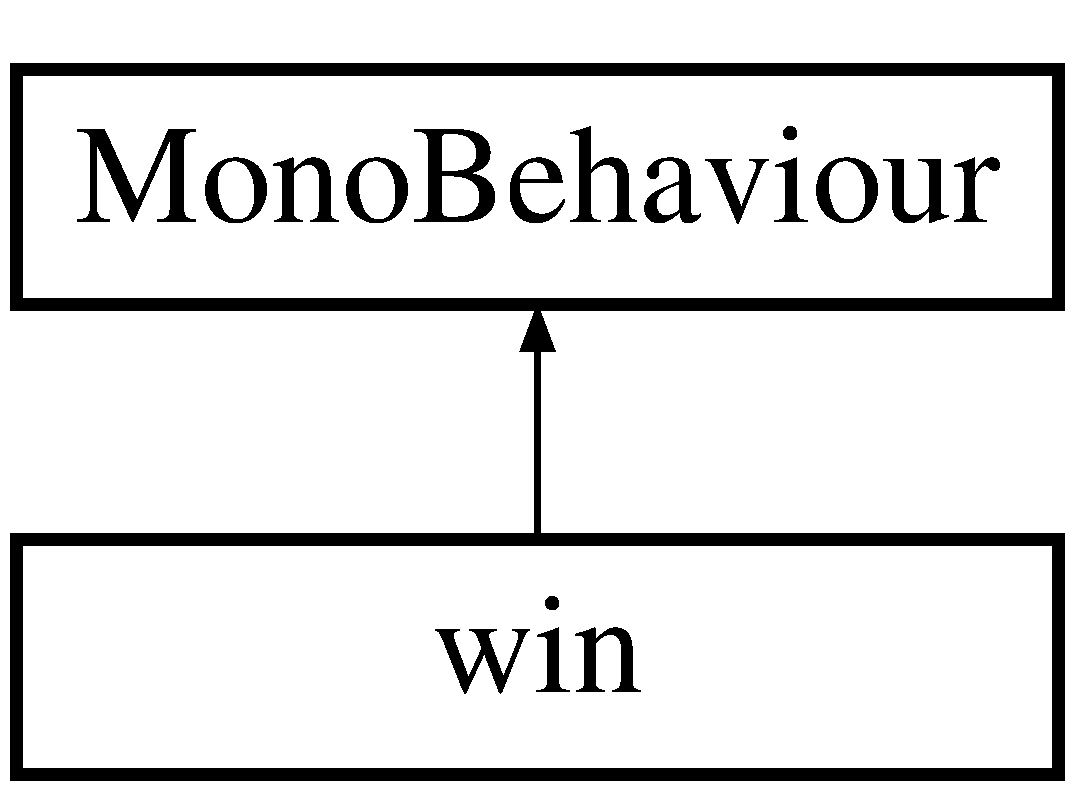
\includegraphics[height=2.000000cm]{classwin}
\end{center}
\end{figure}


The documentation for this class was generated from the following file\+:\begin{DoxyCompactItemize}
\item 
\hyperlink{win_8cs}{win.\+cs}\end{DoxyCompactItemize}

\chapter{File Documentation}
\hypertarget{trigger_8cs}{}\section{trigger.\+cs File Reference}
\label{trigger_8cs}\index{trigger.\+cs@{trigger.\+cs}}
\subsection*{Classes}
\begin{DoxyCompactItemize}
\item 
class \hyperlink{classtrigger}{trigger}
\end{DoxyCompactItemize}

\hypertarget{win_8cs}{}\section{win.\+cs File Reference}
\label{win_8cs}\index{win.\+cs@{win.\+cs}}
\subsection*{Classes}
\begin{DoxyCompactItemize}
\item 
class \hyperlink{classwin}{win}
\end{DoxyCompactItemize}

%--- End generated contents ---

% Index
\backmatter
\newpage
\phantomsection
\clearemptydoublepage
\addcontentsline{toc}{chapter}{Index}
\printindex

\end{document}
